 \chapter{Supplementary charts\label{chap:killer_charts_that_died}}

% \Chapref{chap:killer_charts_that_died} provides addition examples of industries with network effects and/or high regulatory barriers that are highly concentrated. 

% \section{Internet service providers}
\begin{figure}[H]\vspace{2pt}

    \caption{The biggest five banks serve over 80 per cent of the market in most OECD economies \label{fig:5banks}}
    \units{Top five-firm market shares by assets}
    \includegraphics[page=32]{atlas/Charts}
    \notewithsource{Assets of five largest banks as a share of assets of all commercial banks, 2011-2015 average}{Grattan analysis of \textcites{WorldBank-GFDD-2017}{oecd.stat}.
    }
\end{figure}
\begin{figure}[H]\vspace{2pt}

    \caption{Internet service provision is concentrated in most economies \label{fig:ISPs}}
    \units{Top four-firm market shares by subscriptions in internet service providers}
    \includegraphics[page=9]{atlas/ChartsLucy}
    \source{Grattan analysis of \textcites{Statista_ISP_US}{PointTopic_ISP_UK}{Statista_ISP_France}{Statista_ISP_Canada}{Statista_ISP_Australia}{Statista_ISP_Netherlands}}
\end{figure}

\begin{figureTop}
    \caption{Health insurance is frequently a concentrated sector \label{fig:health}}
    \units{Largest firms' market shares by number of people insured in health insurance} 
    \includegraphics[page=18]{atlas/ChartsLucy}
    \noteswithsource{Gradient bars for Belgium, Czech Republic, Netherlands, Chile, Germany and Switzerland show the 2nd and 3rd, and 4th and 5th firms market share as a combined value where individual firm market shares were unavailable.}{Grattan analysis of \textcites{Statista-HealthInsurance-US}{IBISWorldIndustry2017}{KFF-HealthInsurance-US}{OECD-HealthInsurance-2016}}
\end{figureTop}
% \section{General, life and health insurance}

% Three types of insurance are in the top 25 sectors by revenue in Australia. General insurance and health insurance are both highly concentrated (>50\% four-firm market share), and life insurance is moderately concentrated with a 46 per cent four-firm market share.





% Health insurance is hard to compare because most countries have near universal public health care. But there is a small private health insurance market in most OECD countries including Australia (around 10 \% of health expenditure), and a larger market in the US (around 35 \% of health expenditure). %https://theconversation.com/private-insurance-reliance-means-countries-pay-more-for-health-care-24486

% Internationally, there are a mix of very highly concentrated health insurance sectors and some only moderately concentrated countries, \Vref{fig:health}. The US looks relatively unconcentrated compared to Australia at the national level; Australia has a 78 per cent five-firm market share compared to 39 per cent in the US\@. However, at a state level the US is very highly concentrated.

% Florida and Texas are the two states in the US with population closest to Australia's population (20.6 and 27.9 million respectively). Both states have three-firm market shares higher than Australia's five-firm market share.

% \clearpage
\begin{figureTop}
\caption{Insurance sectors are generally concentrated in all countries \label{fig:Insurance}}
\units{Largest firms' market shares by gross written premiums in insurance sectors}
    \includegraphics[page=4]{atlas/ChartsLong_lucy} 
    \noteswithsource{Gradient bars represent 4-firm market shares for life insurance and 5-firm market shares for general insurance where individual firm market shares were unavailable.}{Grattan analysis of \textcites{IBISWorldIndustry2017}{PWC-Insurance-2011}{ABI-Insurance-2007}}
\end{figureTop}
\begin{figureTop}

% Australia's life insurance sector has a relatively low concentration level compared to other high-income countries (\Vref{fig:Insurance}. Spain and Germany are slightly concentrated, although they have much larger populations than Australia does (47 and 80 million, respectively). The UK and France, both larger economies than Australia, are much more concentrated for life insurance.

% For general (or non-life) insurance, Australia has a more concentrated market, but is not an outlier (see also \Cref{fig:Insurance}). For general insurance, economy size seems to have an impact on the level of concentration as larger countries tend to be less concentrated.

% \hl{Concentration in insurance providers is not surprising given inherent business risk. Larger pools of insured persons would smooth the likely payout ratio over time.}
% \clearpage

% \section{Fuel wholesale and retail}

    \caption{Fuel wholesale and retail is also typically concentrated \label{fig:Fuel}}
    \units{Largest firms' market shares in fuel sectors}
    \includegraphics[page=3]{atlas/ChartsLong_lucy} 
    \noteswithsource{Gradient bars for Austria, Turkey and Germany represent 5-firm market share, and for Portugal the 2nd to 4th firm market share, where individual firm market shares were unavailable.}{Grattan analysis of \textcites{OECD-Fuel-2013}{AdC-Fuel-Portugal}{IBISWorldIndustry2017}{Bulgaria_fuel}}
\end{figureTop}

\begin{figureTop}
    \caption{More workers are employed in large firms in higher-income economies\label{fig:firm_employment_size}}
    \units{Employment by firm size, percentage} \vspace{2pt}
    \units{Small firms (1--19 employees)} \vspace{-3pt}
  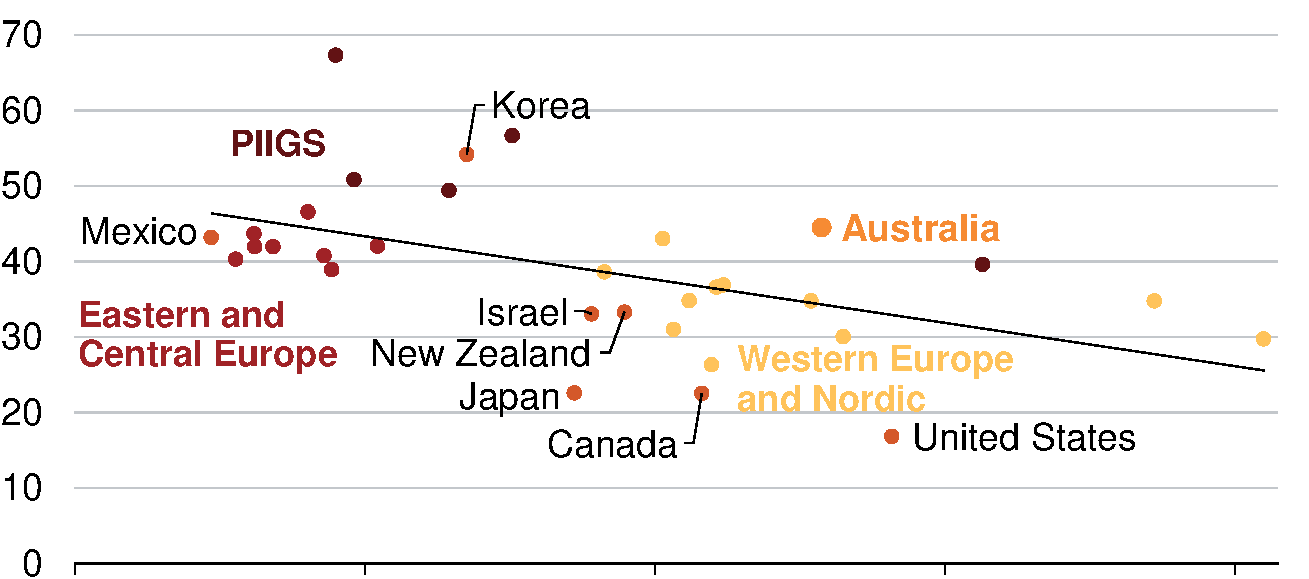
\includegraphics[page=1]{atlas/Fig2_1}
   
  \vspace{5pt}
   
    \units{Large firms (250+ employees)}
  \includegraphics[page=2]{atlas/Fig2_1}
  \notewithsource{GDP per capita based on current exchange rates. OECD countries except Luxembourg. Data for 2014 except Japan (2013) and Israel (2012). Total employment is total number engaged, except in Canada, Korea, and the US (number of employees)% (ISIC Rev. 4)
  . PIIGS: Portugal, Italy, Ireland, Greece and Spain.}{Grattan analysis of \textcite{oecd.stat}.}
\end{figureTop}

% Fuel wholesale and retail tends to be a very highly concentrated industry in most high-income countries. Market power in retail is exacerbated by high levels of vertical integration.%
%     \footcite{OECD-Fuel-2013}

% In Australia, the four largest firms in petroleum product wholesaling have over 90 per cent of the market. Although the data available is limited, it is common for net crude importing countries to have concentrated wholesaling markets (see \Cref{fig:Fuel}).

% Concentration in fuel retailing is also common. In Australia the five-firm concentration ratio is just over 70 per cent, shown in \Cref{fig:Fuel}. In Germany the five-firm concentration ratio is 65 per cent. This is despite Germany having over three times the population and a much more densely populated country.

% In 2013 the OECD conducted a policy round table on competition in road fuel (both wholesale/refining and retail). Submissions from participating countries discuss a consistent list of problems within their borders for these two sectors. In many countries retail and wholesale concentration is worsened by vertical integration between the two sectors.%
%     \footcite{OECD-Fuel-2013}

% Like Australia, many countries also reported have clear ``rockets and feathers'' retail price cycles. Retail prices regularly ``rocket'' up after a market leader makes a move, followed by a period of prices gently falling like ``feathers''.%
%     \footcite{OECD-Fuel-2013}

% Any lack of competitive pressure due to concentration that Australia has in fuel wholesale and retail is shared with many other high-income countries that are net fuel importers.

\begin{figureWhole}
    \caption{Super-normal profits are relatively small across sectors with low barriers to entry \label{fig:low-barriers}}
    \units{Average return on equity in sectors with low barriers to entry, percentage}\vspace{-15pt}
  \includegraphics[page=3]{atlas/ChartsWhole} 
  \noteswithsource{
 Sectors are 4-digit ANZSIC, but some have been aggregated to 2-digit ANZSIC due to size or data limitations. Sector average returns calculated from 2010-11 to 2015-16, excluding goodwill, weighted by firm equity. Shaded areas represent below-normal profits.}{Grattan analysis of \textcites{IBISWorldIndustry2017}{IBISWorldCompany2017}{Morningstar2017}.}
\end{figureWhole}